\documentclass[letterpaper,twocolumn,10pt]{article}
\usepackage{usenix-2020-09}
\usepackage{dirtree}
\usepackage{times}
\usepackage{amsmath}
\usepackage{amsfonts}
\usepackage{pifont}
\newcommand{\cmark}{\ding{51}}%
\newcommand{\xmark}{\ding{55}}%
\usepackage{adjustbox}    % Auto-resize table content
%\usepackage{booktabs}
\usepackage[outputdir=latex.out]{minted}
\usepackage{minted}
\usepackage{graphicx}
\usepackage{listings}
\usepackage{subcaption}
\usepackage{framed}
\usepackage{soul}
\usepackage{textcomp}     % Provides \textmu for upright mu's
\usepackage{tikz}
\usetikzlibrary{positioning}
\usepackage{xspace}
\usepackage{tabularx}
\frenchspacing

% listing styles
\definecolor{codegreen}{rgb}{0,0.6,0}
\definecolor{codegray}{rgb}{0.5,0.5,0.5}
\definecolor{codepurple}{rgb}{0.58,0,0.82}
\definecolor{darkgreen}{rgb}{0.2,0.4,0}
% \definecolor{backcolour}{rgb}{0.95,0.95,0.92}

\usepackage{courier}

\lstdefinestyle{mystyle}{
    % backgroundcolor=\color{backcolour},   
    commentstyle=\color{codegreen},
    keywordstyle=\color{magenta},
    numberstyle=\tiny\color{codegray},
    stringstyle=\color{codepurple},
    basicstyle=\ttfamily\footnotesize,
    breakatwhitespace=false,         
    breaklines=true,                 
    captionpos=b,                    
    keepspaces=true,                 
    numbers=left,                    
    numbersep=5pt,                  
    showspaces=false,                
    showstringspaces=false,
    showtabs=false,                  
    tabsize=2
}
\lstset{style=mystyle}

% And, of course, cleveref must be loaded last-last (read: after hyperref)
\usepackage[capitalise,nameinlink,noabbrev]{cleveref}     % Do the right thing with fig/table references

% Break URLs properly (thanks to Alex Halderman)
\def\UrlBreaks{\do-\do\.\do\@\do\\\do\!\do\_\do\|\do\;\do\>\do\]\do\)\do\,\do\?\do\'\do+\do\=\do\#}
\def\UrlBigBreaks{\do\:\do\/}

%%
\def \gg {\texttt{gg}\xspace}

% comment first line for submission, second line for draft
%\newcommand{\note}[1]{#1}
\newcommand{\note}[1]{}

\newcommand{\shadi}[1]{ {\note{\bf \color{cyan} Shadi: #1}} }
\newcommand{\shadiS}[1]{ {\note{\bf \color{blue} #1}} }
\newcommand{\dhl}[1]{ {\note{\color{red} DHL: #1}} }
\newcommand{\amit}[1]{ {\note{\color{purple} Amit: #1}} }
\newcommand{\seb}[1]{ {\note{\color{darkgreen} Seb: #1}} }


\newcommand{\squishlist}
{
 \vspace*{-0.1cm}
 	\begin{list}{$\bullet$}
		{
			\setlength{\itemsep}{0pt}      \setlength{\parsep}{3pt}
			\setlength{\topsep}{3pt}       \setlength{\partopsep}{0pt}
			\setlength{\leftmargin}{1.5em} \setlength{\labelwidth}{1em}
			\setlength{\labelsep}{0.5em}
		}
	}
	
\newcommand{\squishend}
	{
	\end{list}  \vspace*{-0.2cm}
}


 \newcommand{\squishenum} %Indy
 {
	      \vspace*{-0.2cm}
	      \begin{enumerate}
		     {
			         \setlength{\itemsep}{0pt}
			         \setlength{\parsep}{3pt}
			         \setlength{\topsep}{3pt}
			         \setlength{\partopsep}{0pt}
			         \setlength{\leftmargin}{1.5em}
			         \setlength{\labelwidth}{1em}
			         \setlength{\labelsep}{0.5em}
			     }
		 }
	
	 \newcommand{\squishenumend}
	 {
		     \end{enumerate} \vspace*{-0.2cm}
	 }


\newcommand{\name}{Unum}

%-------------------------------------------------------------------
\begin{document}
%-------------------------------------------------------------------

\date{}

% make title bold and 14 pt font (Latex default is non-bold, 16 pt)
% \title{\Large \bf \name{}: A Library Workflow System for Serverless Applications}
% \title{\Large \bf \name{}: Purely Serverless Workflows with Distributed
% Orchestration}
\title{Doing More with Less: \\ Orchestrating Serverless Applications
without an Orchestrator}

%for single author (just remove % characters)
\author{
  % Paper \#255
{\rm David H. Liu}\\
Princeton University
\and
{\rm Amit Levy}\\
Princeton University
\and
{\rm Shadi Noghabi}\\
Microsoft Research
\and
{\rm Sebastian Burckhardt}\\
Microsoft Research
% copy the following lines to add more authors
% \and
% {\rm Name}\\
%Name Institution
} % end author

\maketitle
\thispagestyle{empty}

\abstract{Workflow systems  have emerged to meet the demands of large-scale serverless
applications with higher-level programming interfaces, rich composition
semantics and strong execution guarantees. However, current designs rely on
%supplemental hosted
centralized orchestrators to execute workflows and thus break out of
the serverless abstraction, compromising key serverless benefits such as fast
auto-scaling, fine-grained billing and efficient resource multiplexing.

This paper presents \name{}, a new design for serverless workflow systems.
In \name{}, a two-stage compiler distributes high-level orchestration
logic to constituent functions at compile-time.
This removes the need for orchestrators at runtime, which allows workflows to
execute purely as serverless functions.
By checkpointing progress to a strongly consistent data store
of choice, \name{} provides strong execution guarantees
and minimizes re-executions under faults.

We present and evaluate an implementation of \name{} that can compile Step
Functions state machines and execute them purely as Lambda functions with
either S3 or DynamoDB as the data store. Our comparison with Step Functions
shows that applications scale up to 4.58x faster and cost more than one
order-of-magnitude less when running with \name{}.
}

%-------------------------------------------------------------------
\section{Introduction}

Serverless computing offers a simple but powerful abstraction consisting of
stateless compute component (Functions as a Service, or FaaS) and scalable,
multi-tenant data stores~\cite{berkeley}. Developers build applications using
task-specific, event-driven ``functions'' without the need to provision or
manage servers. In turn, serverless platforms have been able to offer high
burst-scalability and quickly reclaim function resources as soon as they are
idle. Developers are charged in small compute and storage increments (100s of
milliseconds and per-stored-object and request, respectively), and platforms
can make efficient use of hardware resources.

Originally, serverless platforms targeted simple applications with one or a few
functions and simple interaction patterns. Recently, though, there has been
emerging interest in using serverless platforms to build more complex
applications composed of 10s to 100s functions with rich interaction
patterns~\cite{excamera, pywren, gg-atc, beldi, boki}. Unfortunately, building
such applications using basic serverless building blocks is challenging.
Handling complex control flows and large numbers of functions, in a ad-hoc
manner is difficult to both express and implement correctly.  Additionally, FaaS
invocation semantics requires application developers to gracefully handle
individual function failures and retries.

To meet this need, several workflow systems have emerged to enable serverless
applications with large and complex ``workflows'' of functions. These offer
high-level programming interfaces to express function interactions, supporting a
rich set of composition patterns for chaining, branching, fan-out and fan-in, as
well as exactly-once workflow execution semantics~\cite{excamera, gg-atc,
aws-step-functions, google-cloud-composer, google-workflows, durable-functions}.
These systems rely on some form of \emph{orchestrator} to track workflow
progress, implement interaction logic, and correctly handle retries of
individual steps due to faults or inconsistency in function invocation queues.

An orchestrator is a stateful component that centralizes execution states
and control-flow operations. For each workflow transition in a serverless
application, the orchestrator waits for currently running functions to complete,
determines what to do with their results, and which function(s) to run
next. All function invocations are initiated by the orchestrator, and all
workflow states (e.g., function results) flow through the orchestrator. Using a 
centralized orchestrator simplifies failure handling, as the entire workflow state resides
in the orchestrator and can be easily checkpointed. However, it is also rather
communication-intensive, as all control and data must flow back and forth between
the orchestrator and the functions.

%Such centralized orchestrators enable new classes of serverless applications,
%but requires an additional multi-tenant service to be maintained and operated
%and adds additional contraints on performance and scalability.  
Another downside of many central orchestrators is that they are not serverless themselves.
Commonly, the orchestrator functionality is provided by a separate stateful hosted service
\cite{aws-step-functions, google-cloud-composer, google-workflows}. This requires
development and operation of yet another scalable, multi-tenant, fault-tolerant, 
billable service, in addition to the already existing serverless compute and storage 
infrastructure. 

While basic
serverless build blocks are the result of decades of research and engineering to
achieve performant and scalable compute and storage infrastructure,
orchestrators perform specialized functionality that must solve
scalability and performance problems independently. Applications may suffer, for
example, from scalability bottlenecks in the orchestrator even if storage and
FaaS platforms can support much higher burst-scalability. Moreover, an
orchestrator represents yet-another system for which platform providers must fix
bugs, maintain high availability, and provision resources.

In this paper, \shadiS{we ask a question: \textit{can we achieve the benefits of a workflow  orchestrator, namely ease-of-programming, complex compositions, and failure handling, without having an additional orchestrator service?}}.

We propose \name{}, a \textit{decentralized} serverless workflow system
that runs in-situ with user defined FaaS functions \textit{on existing, minimal,
serverless infrastructure}. \name{} supports the same class of applications as
centralized orchestraters, has similar or better performance, and can achieve
better scalability than some widely used centralized orchestraters. Compared to
Step Functions, a representative set of applications cost up to 32.8x less, and
run up to 4.5x faster using \name{}.

%Importantly, \name{}'s decentralization does not sacrifice properties important
%to complex serverless applications. It can provide the same set of execution
%guarantees as centralized orchestrators. Specifically, \name{} guarantees
%exactly-once execution semantics: even if an application's constituent function
%fails,  is retried, or is otherwise ran multiple times, the final application
%states appear as if all functions executed once.

Importantly, \name{}'s decentralization does not sacrifice any of the  
fault tolerance and strong execution guarantees of 
commonly used orchestrators \cite{aws-step-functions, durable-functions,
 google-cloud-composer, google-workflows}. 
Just like the latter, 
\name{} guarantees that workflows do not get stuck (functions are retried if there are faults)
and produce consistent results (for each constituent function, exactly one result is recorded).
In particular, there is no risk of workflow divergence due to unanticipated function
nondeterminism or concurrency, which is a common source of errors
when developers attempt to compose serverless functions without the help
of a workflow system.

%In particular, for side-effect-free functions, this guaranteeThis matches the guarantees provided by central orchestrators, such as Step Functionsexecution semantics even if an application's constituent function
%fails and is retried or is otherwise run multiple times by the FaaS system.
%Even if some constituent functions execute multiple times, the final application
%states appear as if all functions executed once.

%\dhl{Design insights, highlights and overview}

% \name{} uses a two-stage compiler that tackles the complexity of orchestration
% at compile-time and removes the need to use hosted orchestrator services for
% workflow execution. The compiler transforms workflow definitions (e.g., Step
% Functions state machines) to a continuation-based intermediary representation
% (the \name{} IR \S\ref{sec:design-ir}) and distributes the continuations to
% constiuent functions such that each function is responsible for invoking its
% immediate downstream functions.

% Workflow functions in \name{} are deployed with a runtime wrapper that
% transparently interposes on user code entry and exit. \name{} runtime wrapper
% does not change how users build functions. Developer can still write functions
% exactly the same way as if they are individual functions, and do not need to
% import any additional libraries in order to use \name{}.

% During execution, when user code completes, the runtime wrapper executes the
% assigned continuations which triggers its immediate downstream functions in
% the workflow. Each function performs the same action in the order defined in
% the workflow such that the orchestration logic is distributedly executed by
% the collection of constituent functions.\shadi{this last sentence is a bit vague, reword.}

%  a runtime wrapper transparently interposes on user code
% entry and exit and executes the assigned continuations when user code
% completes. The \name{} runtime wrapper does not change how users build
% functions. Developer can still write functions exactly the same way as if they
% are individual functions, and do not need to import any additional libraries
% in order to use \name{}.

% We present and evaluate an implementation of \name{} that can compile Step
% Functions state machines and execute them purely as Lambda functions using
% either S3 or DynamoDB as the data store. The implementation supports all
% orchestration patterns in Step Functions. Our experimental results show that,
% compared with Step Functions, \name{} improves performance by 11-28\% in the
% case of chaining functions and up to 4.5x in high-parallelism patterns such as
% fan-out. At the same time, \name{} significantly reduces the cost of running
% applications by 3.7x to 32.8x.

This paper makes the following contributions:

\squishlist

  \item An end-to-end system that can take workflows written in high-level
  language and execute them purely as FaaS functions.

  \item A \shadiS{decentralized design for}
  %set of general algorithms, called gadgets, that implement
   all common
  orchestration patterns (e.g., chaining, branching, fan-out, fan-in) using \shadiS{only}
  serverless functions and serverless storage.

  \item An intermediate representation language that can express complex
  workloads in a platform agnostic way, and a front-end
  compiler that transforms Step Functions state machines to the IR.

  \item An implementation of the \name{} runtime that executes workflows purely
  as Lambda functions and uses either S3 or DynamoDB as the data store in order to enable
  fan-in and provide exactly-once semantics. \shadi{this last bullet point is out of place. the first one already mentions system on FaaS. is it trying to highlight the exactly-once? the datastore? or the fact that we have an implementation? }

\squishend
% -------

% execution guarantee challenges.

\section{Background and Objectives}\label{sec:bg}

\begin{table*}[]
\centering
\begin{tabular}{|l|l|l|l|l|}
\hline
 & \textbf{Trigger-based} & \textbf{Driver functions} & \textbf{Orchestrator} & \textbf{unum} \\ \hline
\textit{Purely Serverless}          & \cmark & \cmark & \xmark & \cmark \\ \hline
\textit{Higher-level interface}     & \xmark & \xmark & \cmark & \cmark \\ \hline
\textit{Exactly-once semantics} & \xmark & \xmark & \cmark & \cmark \\ \hline
\textit{Avoid double billing}       & \cmark & \xmark & \cmark & \cmark \\ \hline
\end{tabular}
\caption{Comparison with existing approaches}
\label{table:positioning}
\end{table*}


% Large-scale applications composed of many functions~\cite{excamera, gg-atc,
% deathstar} introduce several new challenges to serverless computing. 

In this section, we describe why it is hard to compose large serverless
workflows, why a purely serverless architecture is interesting and what our
objectives are.

\subsection{Evolution of Serverless Workflows}

\begin{figure}[t!]
    \centering
    \scalebox{.7}{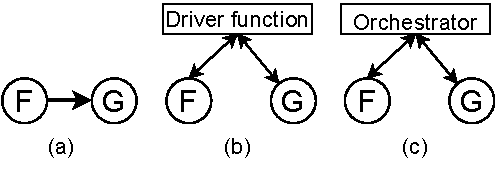
\includegraphics[width=\columnwidth]{figures/ChainExample.pdf}}
    \caption{Chaining two functions with triggers, driver functions and
    orchestrators. In the trigger-based approach, \texttt{F} asynchronously
    invokes \texttt{G} with \texttt{F}'s result. In the driver functions
    approach, a driver function first synchronously invokes \texttt{F},
    usually via HTTP, and after \texttt{F} returns, synchronously invokes
    \texttt{G} with \texttt{F}'s result. Workflow orchestrators provide
    higher-level interfaces (e.g., AWS Step Functions state machines) to
    express function compositions such that \texttt{F}'s code does not contain
    explicit control-flow logic of invoking \texttt{G}. But architecturally,
    orchestrators are similar to driver functions: an orchestrator instance
    invokes \texttt{F}, waits for \texttt{F} to return and then invokes
    \texttt{G} with \texttt{F}'s result.}
    \label{fig:chain-example}
\end{figure}

\subsubsection{Ad-hoc composition: triggers and driver functions}

The original serverless abstraction is designed around developing individual
functions--a \textit{single} unit of work that can run independently on any
machine. However, this design does not provide a higher-level interface to
easily express control-flow logic \emph{between} functions. To build larger
applications that are composed from multiple functions, early adopters use
function invocation APIs to exress control-flows in an ad-hoc manner in one of
the following two ways: \textit{ i. trigger-based}
composition~\cite{netherite} where functions invoke their immediate downstream
functions with \emph{asynchronous} triggers, usually via a queue or data
store, (e.g., a lambda writes to an SQS queue or S3 bucket which in turn sends
an event to Lambda and triggers the next function), and \textit{ii.driver
functions}~\cite{beldi} where a single function, similar to the
\texttt{main()} function of a program, encompasses the control-flow logic and
invokes other functions \emph{synchronously}. Figure~\ref{fig:chain-example}
depicts an example of chaining functions with the two approaches.
	
\shadi{shouldn't the first figure (a) have a storage in the middle?}\dhl{For
the figure, I was intentionally not showing a storage because 1. the point is
that it's \emph{asynchronous}, 2. AWS Lambda's async invoke API actually hides
the fact that it's going over a queue. You simply call \texttt{invoke(data,
RequestType=Event)}, and that adds an item to Lambda's internal queue, which
then generates an event that triggers your lambda. I've adjusted the text to
highlight the \emph{asynchronous} nature and downplay the details about
storage. Take a look and let me know if it works. If not, we can add storage
into Figure 1. But my concern with it is that people might think \name{} needs to
manage similar intermediary data stores while in fact it's managed by Lambda.
The important feature we care about is just that the invocation is
asynchronous. We don't actually care that it's going over a storage.}
\shadi{from the figure and text it is not clear what is the diff between
driver and coordinator. }\dhl{Edited the figure caption. Take a look and let
me know if it's on point and sufficient? High-level note: I think the missing
piece in the text is how the different approaches program differently. How
developers write actual code.}
\shadi {let's just use trigger based throughout the paper}\dhl{Yes.}





%The original serverless abstraction is designed around individual functions
%and does not provide an interface for programming larger applications with
%many functions. As a result, early adopters use low-level function invocation
%APIs to compose functions in an ad-hoc manner, and there are two primary
%approaches.

%The first approach is called trigger-based or unstructure
%composition~\cite{netherite} where functions invoke each other
%\emph{asynchronously} via storage triggers. The second is called driver
%functions~\cite{beldi} where a single \shadi{driver} function invokes other functions
%\emph{synchronously}. Figure~\ref{fig:chain-example} depicts an example of
%chaining functions with the two approaches. \shadi{shouldn't the first figure (a) have a storage in the middle?} \shadi{from the figure and text it is not clear what is the diff between driver and coordinator. }


Although both approaches are ``purely serverless'', i.e., they do not require
adding additional components to the serverless infrastructure, neither is
well-suited for the complexities of emerging serverless applications that
consists of 10s or 100s of functions~\cite{excamera, hello-retail}.
Trigger-based composition scatters control-flow logic across constituent
functions. Development quickly gets unwieldy as the number of functions in the
application increases. More importantly, it does not support all forms of
composition such as fan-in (aggregating results from multiple, potentially
\emph{concurrent} functions after \textit{all} are complete), \dhl{as
asynchronous invocation alone do not support synchronizing across concurrent
instances and can only pass the caller's data, and not other functions' data,
to the callee.}

On the other hand, driver functions concentrate control flow in a single
function and support arbitrary composition. However, they can  create ``double
billing'' by the driver function idly waiting for callees to return. Also, the
driver function has to wait until all functions in the application complete,
which risks hitting the commonly imposed timeouts (e.g., 900 second on AWS
Lambda) and limits scalability.

\shadi{how about the fact that it is sync? doesn't that add delay, e.g., in a
fan-out}\dhl{No, because you can wrap synchronous invocations with async
langugage features locally and batch them. But the driver function still have
to wait for callees to return before proceeding.}

Moreover, neither approach provides the commonly sought-after ``exactly once''
semantics~\cite{netherite, beldi, boki, formal-foundation-exec-gtnee}.
Functions can crash mid-execution due to runtime or hardware faults which may
lead to automatic retries~\cite{aws-lambda-retry, azure-functions-retry}. Even
in the absence of faults, most FaaS systems only ensure at-least-once
execution~\cite{aws-lambda-async-invoke, azure-functions-exec-guarantee}, so a
single invocation can trigger multiple, potentially concurrent, instances.

\shadi{if no failures, why would there be multiple invokes?}
\dhl{Because FaaS engines (e.g., Lambda, Azure Functions) only guarantee
at-least-once execution. So even if you just call \texttt{invoke} once, Lambda
might spin up two instances of the same functions.}
\dhl{Maybe explain why fan-in is not supported as a contrast to \name{}. But
tricky because there's nothing fundamentally stopping unstructured composition
from achieving fan-in as \name{} also demonstrated. Maybe the main difference
is ad-hoc vs ..not. Or maybe the main difference is the addition of strongly
consistent data stores and how we use them.} \shadi{I agree that you should
say why fan-in is not supported. does the current text handle that?}\dhl{Yes
but I'm not confident with the current explanation. Please take a look at the
end of the 3rd to last paragraph. I wrote it in red text.}



%Although both approaches are purely serverless and do not require adding
%additional components to the serverless infrastructure, they each have
%important drawbacks. Unstructured composition scatters control flow across
%constituent functions. As the number of functions increases, development can
%quickly get unwieldy. Moreover, it does not support important composition
%patterns such as fan-in, where we want to invoke a function to aggregate the
%results of multiple upstream functions only after all of them are complete.


%Compared with unstructured composition, driver functions concentrate control
%flow in a single function and supports \shadi{complex patterns such as}aggregation. However, users pay for the
%time when driver functions idly wait for callees to return. This causes
%\emph{double billing}~\cite{double-billing}. \shadi{how about the fact that it is sync? doesn't that add delay, e.g., in a fan-out} Also, serverless platforms
%commonly impose timeouts. A driver function instance has to wait until all
%functions in the application are complete, which risks timeouts and limits
%application scale.

%Moreover, both approaches suffer from weak execution guarantees of the
%underlying serverless system. Functions can crash mid-execution due to runtime
%or hardware faults which may lead to automatic retries~\cite{aws-lambda-retry,
%azure-functions-retry}. Even in the absence of faults, most serverless
%platforms only ensure at-least-once execution~\cite{aws-lambda-async-invoke,
%azure-functions-exec-guarantee} so a single invocation can trigger multiple,
%potentially concurrent, instances. \shadi{if no failures, why would there be multiple invokes?}

\subsubsection{Workflow orchestrators}

Recently, workflow orchestrators have emerged to tackle the challenges of
large serverless applications~\cite{excamera, gg-atc, aws-step-functions,
google-cloud-composer, google-workflows, durable-functions}. Orchestrators are
separate hosted services that execute workflow definitions, invoke constituent
functions and manage workflow states. Architecturally, they are similar to
driver functions (Figure~\ref{fig:chain-example}). For every workflow
invocation, an orchestrator instance invokes a constituent function, waits for
its result and passes it to downstream functions via invocation. All functions
invocation are initiated by the orchestrator and all states (e.g., function
results) pass through the orchestrator.

Different from ad-hoc composition, orchestrators offer (1). higher-level
programming interfaces that directly express function interactions and hide
low-level APIs, (2). a rich set of composition primitives, including
branching, chaining, fan-out and fan-in, (3). exactly-once semantics for
workflow execution, and (4). long or no runtime limits.

While fixing the flaws of ad-hoc composition, the orchestrator design creates
several important drawbacks that neglect or even compromise key benefits of
the serverless abstraction: (1). End-to-end performance now also depends on
the orchestrator service that is separate from the FaaS engine. A slow
orchestrator can become a bottleneck and nullify the fast autoscale advantage
of serverless. (2). Serverless computing already offers compute and storage
building blocks that are highly performant and scalable. Adding yet another
separate service that is a mixture of compute and storage is repeating the
difficult and expensive task of developing and maintaining a large-scale system,
which often requires a dedicated engineering team.(3). Platform-specific
orchestrators force developers to write with proprietary APIs and locks them
in a particular cloud provider.\dhl{I'm hesitant to include the 3rd point
because 1. we can't demonstrate that \name{} solves this problem. 2. while
it's a benefit, it feels more an engineering problem than a research problem.
3. FaaS functions are already platform-specific. Lambda, Azure functions, etc.
all have different propritary APIs.} \shadi{I thought the point here was to be a design goal of "interoperability".}
\dhl{Yes, but the problem is that current \name{} implementation only works on AWS. So we can't show/prove that we achieved interoperability if we list that as a goal. }

\subsection{Research question and objectives}

In this paper, we examine whether we can have the best of both worlds. We
argue that it is possible to preserve the advantages of workflow orchestrators
while building entirely on top of the existing serverless computing
abstraction without adding any supplemental components.

Specifically, we aim for a system with the following objectives:

\paragraph{\emph{Purely serverless}} The system should work within the current
serverless environment and not require adding any new services.

The system should execute workflows solely as event-driven serverless
functions, and use serverless storage, when necessary, to enable stateful
operations (e.g., fan-in).

\paragraph{Higher-level programming interface} Developers should express
function compositions with higher-level primitives similar to exising workflow
orchestrators (e.g., AWS Step Functions) instead of ad-hoc mechanisms.

\paragraph{Supports all common interactions} The system should support all
composition patterns commonly used in orchestrators today, including chaining,
branching, fan-out and fan-in.

\paragraph{Exactly-once semantics} Even if a function executes multiple times,
due to retries or duplicate invocations, concurrently or non-concurrently, the
final state should appear that the execution happened only once.

\paragraph{Avoids double billing} Users should only pay for the resources
used. Functions should not synchronously wait for other functions to return.

\paragraph{Comparable performance and costs} The system should at least have
comparable costs and performance as the state-of-the-art workflow
orchestrators.

\section{Design}\label{sec:design}

\name{} is an application-level orchestration system that supports complex
serverless applications without a standalone orchestrator. It does so by
decentralizing orchestration logic in a library that runs in-situ with
user-defined FaaS functions and leverages a scalable consistent data store for
coordination and execution correctness. By removing standalone orchestrators,
\name{} improves application flexibility and reduces costs. Importantly,
\name{} does this while retaining the expressiveness and execution guarantees
(\S\ref{sec:design:execution}) of standalone orchestrators.

\subsection{Architecture}\label{sec:design:architecture}

\begin{figure*}[t!]
	\centering
	\begin{subfigure}[t]{0.8\textwidth}
	\centering
		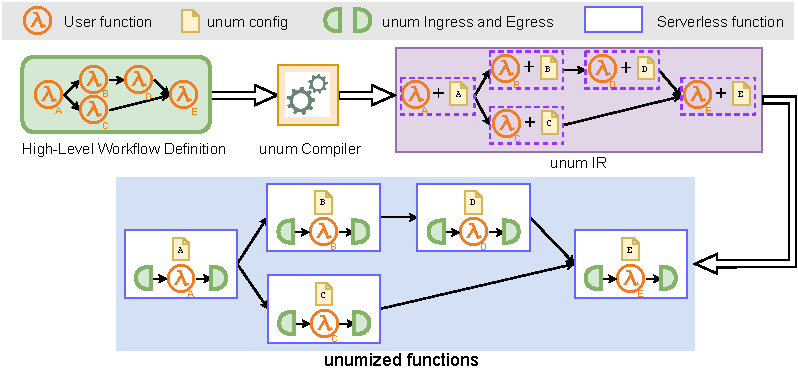
\includegraphics[width=0.8\columnwidth]{figures/unum-arch-compile-time.pdf}
		\caption{Serverless workflows form directed graphs. \name{}
		partitions the graph into an intermediate representation where each
		function is embedded with an \name{} configuration that encodes how to
		transition to its immediate downstream nodes. Developers package user
		function, \name{} config and \name{}'s runtime library (a pair of
		ingress and egress components) together to create ``unumized'' functions.}
		\label{fig:arch:unum-compile-time}

	\end{subfigure}
	\begin{subfigure}[b]{\columnwidth}
		\centering
		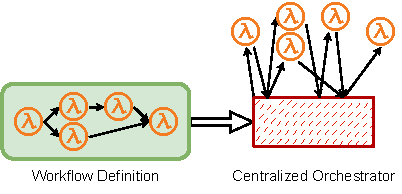
\includegraphics[width=0.8\columnwidth]{figures/unum-arch-centralized.pdf}
    \caption{A typical standalone orchestrator operates as a logically
    centralized controller that drives the execution of applications by
    invoking functions, receiving function results and storing application
    states}
    \label{fig:arch:centralized}
	\end{subfigure}
	\hfill
	\begin{subfigure}[b]{\columnwidth}
		\centering
		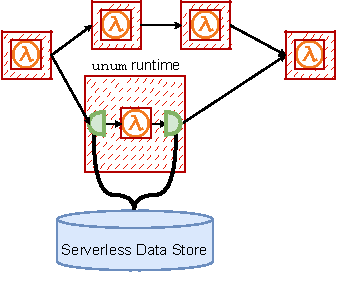
\includegraphics[width=.7\columnwidth]{figures/unum-arch-runtime.pdf}
		\caption{At runtime, \name{} orchestration logic is decentralized and
			runs in-situ with the user functions on an unmodified serverless
			platform. For coordination and checkpointing,
			\name{} relies exclusively on a standard data store of choice, such
			as DynamoDB or Cosmos DB.}
		\label{fig:arch:unum-runtime}
	\end{subfigure}
	\caption{\name{}'s Decentralized Orchestration. \name{} partitions
	orchestration logic at compile time and a \name{} runtime runs in-situ
	with user functions to perform only the orchestration logic local to its
	node.}
	\label{fig:arch}
\end{figure*}

Figure~\ref{fig:arch:unum-compile-time} depicts how developers run serverless
workflows using \name{}. Developers write individual functions and describe the
workflow using a high-level workflow language, such as Step Functions'
expression language. An \name{} front-end compiler uses these to extract
portable \name{} IR for each node in the graph and ``attaches'' it to the
function (e.g.\ by placing a file containing the IR alongside the function
code). A platform-specific \name{} linker ``links'' each function with a
platform-specific \name{} runtime library.~\footnote{Since functions are
typically written in dynamic languages, the \name{} library source code is
placed alongside the function and dynamically imported, rather than statically
linking an object file} Developers deploy each linked function along with its IR
to the FaaS platform.

Each \name{} workflow begins with an ``entry'' function. Invoking this
function (e.g.\ using an HTTP or storage trigger) starts a workflow. Moreover,
admission control rules for the workflow, such as access control and rate
limiting, are implemented by setting appropriate rules on this entry function.
For example, a workflow can be invoked by a particular principal if the entry
function is exposed to that principal.

The runtime library is composed of an ingress and egress component that run
before and after the user-defined function and unwrap and wrap the results of
the function in \name{} execution state, respectively
(Figure~\ref{fig:design:unum-request}). The ingress component coalesces input
data from each incoming edge (e.g.\ in a fan-in), resolves input data if passed
by name rather than by value, and passes the input value to the function. The
egress component uses the function's result to invoke the next function(s),
enforces execution semantics using checkpoints, performs coordination with
sibling branches in fan-in, and deletes intermediate states no longer needed for
the workflow, executing the workflow in-situ with the functions, in lieu of a
centralized orchestrator (Figure~\ref{fig:arch:unum-runtime}).



\subsection{\name{} Intermediate Representation}\label{sec:design:ir}

\begin{table}[t]
  \centering
  \begin{tabular}{|m{0.45\linewidth}|m{0.45\linewidth}|}
    \hline
  \texttt{Invoke(Fn)} & Queue a single invocation of a function.\\
    \hline
  \texttt{Map(Fn)} & Queue one function invocation for each element in the current function's result.\\
    \hline
  \texttt{FanIn(Set, Size, Fn)} & Queue a fan-in to a function using the provided coordination set object and size.\\
    \hline
  \texttt{Pop} & Pops the top frame of the execution state stack (passed via \name{} requests). \\
    \hline
  \texttt{Next} & Increments the current execution state frame's iteration counter.\\
    \hline
  \texttt{CreateSet(Name)} & Creates a coordination set object in the data store with the provided name.\\
    \hline
  \end{tabular}
  \caption{\name{} intermediate representation instructions.}
  \label{table:design:irschema}
\end{table}

\begin{figure}[t]
    \centering
    \begin{minted}[
        frame=single,
        fontsize=\scriptsize
        ]{rust}
struct InvocationRequest {
  data: Vec<DatastoreObjectName>,
  workflowId: String,
  fanOut: Stack<FanOut>,
}

struct RequestData {
  reference: DatastoreObjectName,
  value: Option<Value>
}

struct FanOut {
  index: usize,
  size: usize,
  iteration: usize,
}
    \end{minted}
    \caption{An \name{} request wraps the outputs of parent nodes with execution
state that allows function invocations to be named uniquely and assists in
coordinating fan-ins. \name{} IR instructions can reference this metadata and
modify it for subsequent functions.}
    \label{fig:design:unum-request}
\end{figure}

Similar to many standalone orchestrators, \name{} applications are modeled as
directed execution graphs where nodes represent user-defined FaaS functions
and edges represent function invocations (incoming edges) with the output of
one or more other functions (outgoing edges).

An \name{} graph may include fan-outs, where a node's output is used to invoke
several functions or split up and ``mapped'' multiple times on the same
function. Each such branch may be taken conditionally, based on the output
value or dynamic states of the graph. Execution graphs may also contain
fan-ins, where the outputs of multiple nodes are used to invoke a single
aggregate function. Cycles are also supported and each iteration through a
cycle is a different invocation of the target function.

The \name{} intermediate representation (IR) is designed to encode directed
execution graphs in a way that both allows decentralization of orchestration
and is low-level enough to support application-specific patterns.

Each function's IR includes the function's name and a sequence of instructions
(Table~\ref{table:design:irschema}). Instructions direct the runtime to invoke
functions and operate on state metadata passed between functions in
\name{}-wrapped function inputs (Figure~\ref{fig:design:unum-request}).

The egress component, which receives the function's user-code output, executes
the IR and uses it to determine which next steps to take. An invocation can be
protected by a conditional---a boolean expression that operates on the
invocation request and the current function's output. \name{}'s IR provides
three kinds of invocations:

\begin{itemize}
  \item \textbf{Invoke} simply invokes the named function using the
        current functions output.
  \item \textbf{Map} treats the current function's output as iterable data
        (e.g.\ a list) and invokes the named function once for each item in the
        output.
  \item \textbf{FanIn} invokes the named function using the current function's
        output along with the outputs of all other functions fanning into the
        same node. Fan-in requires coordination among multiple functions and is
        described in detail in \S\ref{sec:design:fanin}.
\end{itemize}

When multiple invocations occur, either using multiple instructions or a single
\texttt{Map} invocation, each of the invocations adds a fan-out frame to the
invocation request's fan-out stack. This allows different invocations of the
same function to be differentiated for naming (\S\ref{sec:design:naming}) and to
coordinate fan-in (\S\ref{sec:design:fanin}).

The IR also includes instructions for manipulating the \name{} request data and
an instruction that creates a new coordination set, typically for use in later
nodes to coordinate fan-in (\S\ref{sec:design:fanin}) or garbage collection
(\S\ref{sec:design:garbage}).

This IR is sufficient to represent basic patterns, as well as more complex
fan-in patterns (described in \S\ref{sec:design:fanin}).

\paragraph{Chain \& Fan-out.}
\name{} encodes passing the output of a function to one (chaining) or more
(fan-out) subsequent functions, simply, with one or more calls to the
\texttt{Invoke} instructions.

\paragraph{Map.}
Applications may also perform the same operation on each component of a
function's output. For example, an application may unpack an archive of
high-resolution images in one function and perform compression on each of the
resulting images. \name{}'s \texttt{Map} invocation pass each element from the
function's output to a different invocation of the same function.

\paragraph{Branching.}
Applications may need to invoke different functions based on runtime conditions
(e.g., the output of a function). For instance, an application may first
validate that a user-uploaded photo is a valid JPEG. If it is, it invokes, e.g.,
one of the patterns above, otherwise it notifies the user of the error.
\name{}'s invocation instructions are optionally protected by a conditional
expression that has access to the function output and execution metadata
(Figure~\ref{fig:design:unum-request}).



\subsection{Execution Guarantees Using Checkpoints}\label{sec:design:execution}

FaaS functions only provide weak execution guarantees. Functions can fail
mid-execution and be retried. Even in the absence of failures, one function
invocation may result in more than one execution because most FaaS engines
only ensure at-least-once execution. This is problematic for applications
whose functions are non-deterministic because a single workflow invocation can
produce multiple \emph{diverging} outputs.

An important benefit of orchestrators is strong execution semantics such that
applications appear to execute \emph{exactly-once} even if individual
functions in the application run multiple times. Because standalone
orchestrators are logically centralized, guaranteeing exactly-once is
conceptually straightforward: the orchestrator can choose a single result from
executions of the same invocation and use it as input for all downstream
functions. At the end of the workflow, the result is consistent with an
execution of the workflow where each function invocation executed
exactly-once.

A key challenge for \name{} is to provide the same semantics without
centralizing orchestration. Moreover, because failures and, thus, retries are
the exception, not the rule, \name{} should provide these semantics without
expensive coordination---function instances should be able to proceed without
blocking in the common, fault-free case.

\name{} leverages two key insights to achieve these semantics.  First, it is
 correct for different executions of the same function invocation to return
 different results as long as \name{} ensures downstream functions are always
 invoked with exactly one of those results. Second, a workflow's output is
\emph{correct} even if a function is invoked more than once, as long as the
invocations uses the same input, since additional, but identical, invocations
are indistinguishable from additional executions.

The \name{} library employs an atomic \texttt{create\_if\_not\_exists}
operation in the serverless data store to \emph{checkpoint} exactly one
execution of each function invocation. The egress component of the \name{}
library attempts to write the result of the function to a checkpoint object in
the data store. If such a checkpoint already exists, a concurrent or previous
execution of the invocation must have already completed and the operation will
fail. To invoke downstream functions, the egress component \emph{always} uses
the value stored in the checkpoint, rather than the result of the recently
completed function. Essentially, \name{} ``commits'' to result of the first
successful executions of invocations.

Data stores need to be strongly consistent to support
\texttt{create\_if\_not\_exists}. It is important that a later attempt to
create an existing checkpoint fails and the slower execution can read the
existing checkpoint.

As a further optimization, the ingress component in the \name{} library checks
for the checkpoint object before executing the user-defined function. If the
object exists, it bypasses the user-defined function and passes the checkpoint
value directly to the egress component to invoke downstream functions. This is
not necessary for correctness (and it is, of course, possible for the checkpoint
to be added after a concurrent execution checks for its existence in the ingress
component) but helps reduce computation that we know will go unused.

Note that the exactly-once guarantee does not automatically extend to
applications with external side effects, i.e. functions that directly call
external services. In such cases, retries can lead to unexpected results if
the effects are not idempotent. This issue is well known, and independent of
the orchestrator architecture (centralized vs. decentralized). Thus, we
consider the question of how to control such side effects to be orthogonal and
beyond the scope of this paper. However, \name{} does not preclude
applications from using libraries, such as Beldi~\cite{beldi}, that can solve
this problem.

% \begin{table}
%   \centering
%   \begin{tabular}{|m{0.18\linewidth}|m{0.73\linewidth}|}
%     \hline
%   \textbf{Workflow} & A directed graph of functions that takes an input and produces one or more outputs. \\
%     \hline
%   \textbf{Function} & A user-defined FaaS function, linked with the \name{} runtime library. \\
%     \hline
%   \textbf{Invocation} & An request to the FaaS platform to run a function. \\
%     \hline
%   \textbf{Execution} & The FaaS platform may attempt to \emph{execute} a function invocation one or more times, and guarantees that at least one execution completes. \\
%     \hline
%   \end{tabular}
%   \caption{\name{} terminology.}
%   \label{table:terms}
% \end{table}


\begin{figure}
\begin{minted}[
    frame=single,
    fontsize=\scriptsize
    ]{python}
def ingress(self, function):
    ...
    result = datastore_get(self.checkpoint_name):
    if result:
        self._egress(result)
    else:
        self.egress(function.handle())

def egress(self, result):
    ...
    if not datastore_atomic_add(self.checkpoint_name, result):
      result = datastore_get(self.checkpoint_name)
    self._egress(result)
    ...

def _egress(self, result)
    for f in next_functions:
        faas.async_invoke(f, result)
\end{minted}
\caption{Pseudo-code showing \name{}'s checkpointing mechanism. As different
executions of a function may return different results, \name{}'s egress
component checkpoints the first successful execution using an atomic add
data store operation. All subsequent executions will uses this committed value
rather than the result their own execution returned.}
\label{fig:design:checkpoint}
\end{figure}

\subsubsection{Fault Tolerance}

Another source of multiple executions is retrying failed functions. Retries in
\name{} rely on FaaS engines' error handling support. All popular FaaS engines
provide error handling so that applications do not just crash silently without
a way to react to failures. Common mechanisms include ``automatic retry'' that
re-executes the same function~\cite{aws-lambda-retry, azure-functions-retry,
google-cloud-functions-retry, openfaas-retry} or failure redirection that
triggers a pre-configured error-handler
function~\cite{aws-lambda-failure-destination,
openwhisk-action-error-handling}. \name{} can work with either mechanism.

The \name{} error handler is part of \name{}'s standard library and is
triggered in a separate FaaS function after an application function crashes.
The error handler simply retries the crashed function by invoking it again. As
part of the orchestration library, the error handler is assumed to be bug-free
and relies on the FaaS scheduler to execute at least once.

\name{}'s checkpointing mechanism ensures that while faults may occur at any
point during the execution of a function's user code or the \name{} library,
and while downstream functions may be invoked multiple times by different
executions of the same invocation, a single value is always used to invoke
downstream functions.

If there is a fault after the user code completes but before creating the
checkpoint, user code result is ignored (indeed, never seen) by other
executions and another execution's value will be used to invoke downstream
functions.  If the ``winning'' function crashes after creating a checkpoint,
and before invoking some or all downstream functions, other executions will
use the checkpoint value to invoke downstream functions. Finally, even if
multiple executions invoke some or all downstream functions, execution
guarantees are still satisfied as these invocations will have identical
inputs.

% Retries in \name{} rely on FaaS engines' error handling support. All popular
% FaaS engines provide error handling so that applications do not just crash
% silently without a way to react to failures. Common mechanisms include
% ``automatic retry'' that re-executes the same function~\cite{aws-lambda-retry,
% azure-functions-retry, google-cloud-functions-retry, openfaas-retry} or
% failure redirection that triggers a pre-configured error-handler
% function~\cite{aws-lambda-failure-destination,
% openwhisk-action-error-handling}. \name{} just needs a way to regain control
% on the application-level and can therefore work with both mechanisms.

% When a function crashes, the FaaS engine retries the failed function or direct
% the error to \name{}'s error handling function. In either case, the \name{}
% runtime in the new execution checks the nature of the failure and, if a
% re-execution is necessary, invokes the failed function again. The error
% handling function itself does not run user code. In other words, \name{} does
% not rely on FaaS engine's automatic retry mechanism for re-executing failed
% functions; it only uses automatic retry to run the error handling
% functionality in the \name{} runtime which in turn manually retries failed
% function by invoking it. This enables \name{} to circumvent potential
% limitations on FaaS engine's automatic retry mechanism\footnote{For instance,
% Lambda's automatic retry only retries up to 3 times}. As long as a FaaS engine
% allows applications to run error handle code in response to failures, \name{}
% retry can work.

\subsection{Fan-in Patterns}\label{sec:design:fanin}

In fan-in patterns, the results of multiple nodes are used to invoke a single
target node. Such patterns are a particular challenge for decentralized
orchestration because invoking the target function cannot happen until all
branches complete, but there is no standalone orchestrator to wait for this
condition. Designating one of the dependent functions as a coordinator for
the fan-in would address this directly. However, there is no guarantee that
branches for a fan-in complete soon after each other, incurring a potentially
large resource cost to do virtually no work, and risk exceeding
platform-enforced function timeouts. Moreover, functions typically cannot
communicate with each other directly, so it is not obvious how other branches
would notify this coordinator of their completion.

\name{}, instead, leverages the same insight as checkpoints---the data store
provides strong consistency that can serve as a coordination point. Rather
than designating a single branch function as the coordinator, all branches are
empowered to invoke the fan-in function once all other branches have
completed. To determine this condition, branches in a fan-in add the name of
their checkpoint object to a shared ``Set'' in the data store. Any branch that
reads the set with size equal to the total number of branches invokes the
target function using all the branches' checkpoints as input.

Importantly, functions do not wait for any other to complete. As long as all
functions complete eventually (in other words, they run at-least once),
\emph{some} function will read a full set and invoke the fan-in target
function. More than one function may observe this condition, resulting in
multiple invocations, but these invocations will be identical and are handled
as spurious executions of the same invocation (\S\ref{sec:design:execution}).

In order to perform this coordination, branches must know the branching
factor---the size of the set. The \texttt{FanIn} instruction includes this
size, which is either specified explicitly, or using a variable from the
invocation request, commonly the fan-out size.

Similar to checkpoints, the set data structure for coordination requires the
data store to be strongly consistent. Updates to a set must be immediately
visible to other branches otherwise the downstream fan-in function may ever be
invoked. Moreover, the data store must support data structures that can
implement a ``set'' abstraction.

Fan-in supports enable more patterns that commonly arise in applications:

\paragraph{Aggregation}
After processing data with many parallel branches, applications commonly want to
aggregate results. For example, to build an index of a large corpus, the
application might process chunks in parallel and then aggregate the results.
Aggregation is a common pattern to join back multiple parallel functions, by
invoking a single ``sink'' function with the outputs from a vector of functions.

\paragraph{Fold}
\texttt{fold} sequentially applies the same function on the outputs of a vector
of source functions, while aggregating with the intermediate results of running
the function so far. For example, a video encoding application might encode
chunks in parallel and then concatenate the results in order: concatenating
chunk 1 and 2, then concatenating chunk 3 to chunk [1--2], and so on.
\texttt{fold} is an advanced pattern that is not supported by all existing
systems (e.g., AWS Step Functions do not support \texttt{fold}) but is
expressible in \name{}.


\subsection{Garbage Collection}\label{sec:design:garbage}

Both checkpointing and fan-in require storing intermediate data (e.g.,
checkpoints and coordination sets) in the data store. These intermediate data
is only temporally useful and grows with each invocation. This poses a garbage
collection challenge. Deleting them too early can compromise execution
guarantees while deleting too late incurs storage costs.

As an application-level library, \name{}'s design allows applications to
customize their GC strategy. Simple policies such as deleting intermediate
data older than a set limit are easily implementable via data stores or as a
cron job. However, in this section, we demonstrate the algorithm in \name{}'s
standard library that deletes checkpoints and coordination sets \emph{as soon
as} they are no longer needed for execution correctness, to show that
\name{}'s decentralized design allows the most aggressive strategy.

\subsubsection{Checkpoint Collection}

A checkpointing node does not know when \emph{its} checkpoint is no longer
necessary.  If it deletes its checkpoint after invoking subsequent functions but
before completing, it may crash and the FaaS platform may re-execute it,
yielding a potentially inconsistent result. However, downstream nodes know that
once they have committed to a value by checkpointing, previous checkpoints are
no longer necessary to ensure their own correctness. Once a node has committed
to some particular output, future invocations, even with \emph{different} inputs
will produce the same output, as the node will \emph{always} use the checkpoint
value.

Note that a duplicate execution that checkpoints after the previous checkpoint
is garbage collected has the same semantics as a separate invocation. It may
result in multiple outputs from the workflow, though each output is still
consistent with an execution of the workflow where each function was invoked
exactly-once. Any GC policy, no matter how conservative, might lead to
multiple executions if the FaaS platform might execute duplicates of a
function invocation an arbitrary time in the future.

In particular, \name{} collects checkpoints by relaxing the constraint that
nodes always output the same value. Instead, they must only output the same
value until all subsequent nodes have committed to their own outputs. This
means that, in non-fan-out cases, once a node checkpoints its result, it can
delete the previous node's checkpoint.

\name{} runtime implementations delay garbage collection until after invoking
next functions, sacrificing some storage overhead in favor of minimizing
end-to-end latency for a workflow.

Fan-out cases are more complicated because deleting the checkpoint must wait
until all branches have committed to an output. \name{} repurposes the same
set-based technique from fan-in to collect checkpoints in fan-out cases as
well. The originating node of a fan-out creates a set for branches to
coordinate when to delete its checkpoint. Branches add themselves to the set
after checkpointing their own value. Any node that reads a full set deletes
the parent's checkpoint as well as the set. This guarantees that the parent's
checkpoint is deleted and ensures that all branches have first checkpointed.

Note that it is possible for one of the branches to re-execute \emph{after}
the set has been deleted. This is safe because it is the origin of the fan-out
that creates the set, so a branch's attempt to add itself to a, now,
non-existent set will simply fail.

% \begin{minted}[
%     frame=single,
%     fontsize=\scriptsize
%     ]{python}
% def egress_fan_out(self, result):
%     result = _checkpoint(self, result)
%     _do_next(result)

%     completion_set_after =
%         write_set_read_result(fan_out_gc_set, fan_out_index)
%     if all_complete(completion_set_after):
%         database_delete(prev_checkpoint)
%         database_delete(fan_out_gc_set)
% \end{minted}

\subsubsection{Fan-in Set collection}

Deleting sets used for fan-in works much like removing checkpoints---the
target node of a fan-in deletes the set once it has generated a checkpoint.
However, who \emph{creates} the set?

If each branch in the fan-in creates the set if it doesn't already exist, a
spurious execution of one of the branches \emph{after} the fan-in target
removes the original set will create a new one that is never deleted (because
it never fills, and thus the target function is never invoked again). To avoid
this, \name{} places the responsibility to create the set on the node that
originates the \emph{fan-out} at the same level as the target node.

\subsection{Naming}\label{sec:design:naming}

Much of \name{}'s functionality relies on unique naming. A workflow invocation
must be named to differentiate it from other concurrent invocations of the
workflow; functions must be named to invoke them; different invocations of
functions must have different names to uniquely name invocation checkpoints
and coordination sets for fan-in.

Each workflow invocation has a unique name that is passed through the
execution graph. The name is either generated in the ingress to the first
function using, e.g., a UUID library or, when available, is taken from the
FaaS platform's invocation identifier for the first function. This enables
functions to have different names when invoked as part of a specific workflow
invocations. The function's name is either user-defined or determined by the
FaaS platform (e.g.\ the ARN on AWS Lambda) and determined at ``compile-time''
(i.e.\ when generating \name{} IR).

However, this is not sufficient as functions may be invoked multiple times in
the same workflow due to map patterns---which invoke the same function
multiple times over an iterable output---and cycles. Moreover, invocation
names must be determined using local information only. Once running, each
function only has access to it's own code (including the IR) and metadata
passed in its input. Nonetheless a particular invocation must be able to
determine its own name for checkpointing as well as, if it is part of a
fan-in, the name of downstream invocations to coordinate with other branches.

As a result, \name{} names function invocations using a combination of the
global function name, a vector of branch indexes and iteration numbers (taken
from the \name{} request fan-out stack) leading to the invocation, and the
workflow invocation name. Function names are global and the remaining items
are propagated by \name{} in invocation arguments.

During a fan-out pattern (multiple scalar invocations or a map invocation), a
branch index is added to a list in the next functions' input. If the next
function is an ancestor of the current function (a cycle), an iteration field
in the input is incremented. Note that a single iteration field is sufficient
even if there are nested cycles since it is only important that different
invocations of the same function have \emph{different} names, not that the
iteration field is sequential. Thus, a monotonically increasing iteration
field is sufficient.

We note that the format of this name is not significant and, importantly, it
need not be interpretable. It must only be deterministic and unique for its
inputs. For example, a reasonable implementation could serialize the inputs
and take a cryptographic hash over the result, guaranteeing uniqueness (with
very very high probably) while preventing names from growing too large to use
as object names.

\section{Implementation}\label{sec:impl}

We implement a prototype \name{} runtime that supports AWS Lambda and Google
Cloud Functions, leveraging DynamoDB and Firestore, respectively, as
intermediate datastores. We also implemented a front-end compiler that takes
arbitrary AWS Step Function state-machine definitions and compiles them to
\name{} IR, which can be run on either. Currently our runtime only supports
Python functions and is itself written in 1,119 lines-of-code. The Step
Functions compiler is 549 lines-of-code.

Implementing the runtime primarily requires specializing high-level
functionality the IR depends on for a particular FaaS platform and datastore.
The FaaS platform must support asynchronous function invocation and the
datastore must be linearizable with support for atomic creation and set
operations.

Importantly, we choose datastores and primitives that only incur per-use costs,
rather than including baseline provisioning cost, and scale on-demand. For
example, we use DynamoDB in on-demand capacity mode, rather than provisioned
capacity mode, and avoid long-running services such as a hosted Redis or cache.
As a result, \name{} workflows, like their centralized counterparts, incur
resource costs \emph{only} to actually execute a workflow.

\subsection{AWS Lambda \& DynamoDB}

Asynchronous invocation in Lambda is natively supported. In particular, the
Lambda \texttt{Invoke} API is asynchronous when passed
\texttt{InvocationType=Event}. \majoredits{In the event of a crash, we use
Lambda's Failure Destination~\cite{aws-lambda-failure-destination} to redirect
the fault to an error handler function which runs just the \name{} runtime.
The error handler checkes if the failed function should be retried (e.g.,
based on the Step Function definition~\cite{aws-step-functions-retry}) and if so,
retries the function by explicitly invoking it again.}

DynamoDB organizes data into tables, with each item in a table named by a key.
Within tables, items are unstructured by default. Our implementation of
\name{} uses a single table for each workflow. Each item in the table
corresponds to a checkpoint, or a coordination set for fan-in or garbage
collection.

DynamoDB supports atomic item creation by passing the conditional flag
\texttt{attribute\_not\_exists} to the \texttt{put\_item} API call. We use
this for creating both checkpoint blobs and coordination sets. DynamoDB
supports set addition natively using the \texttt{Map} field type. In
particular, we use update expressions to atomically set a named map element to
true.  As an optimization, we use the \texttt{ALL\_NEW} flag when adding to a
set to atomically get the new value after a set in a single operation.

\subsection{Google Cloud Functions \& Firestore}

Google Cloud Functions (GCF) do not have an asynchronous invocation API.
Instead, we allocate function-specific pub-sub queues and subscribe each
function to its respective queue.  \name{} then asynchronously invoke a
function by publishing the input data as an event to the function's queue.

\majoredits{GCF supports automatic retry for asynchronous
functions~\cite{google-cloud-functions-retry}. In the event of a crash,
\name{} runtime in the retry execution checks if the failed function should be
retried and if so, retries the function by explicitly invoking it again.}

Firestore organizes data into logical collections (which are created and
deleted implicitly) containing unstructured items, named by a unique key.
Similar to DynamoDB, we use a separate collection for each workflow. Atomic
item creation is supported using a special \texttt{create} API call, which
only succeeds if the key does not already exist. Firestore supports an
\texttt{Array} field type which can act as a set by using the
\texttt{ArrayUnion} and \texttt{update} operation, which atomically sets the
field to the union of its existing elements and the provided elements. The
\texttt{update} operation always returns the new value data.


\section{Evaluation}\label{sec:eval}

We evaluate \name{} along 3 metrics: (1). cost, (2). latency, and (3).
expressiveness, to answer the following questions:

\begin{enumerate}

    \item What is the cost of running applications on \name{} and how does it
    compare to existing serverless workflow systems? Specifically, how much
    additional costs does the \name{} runtime incur in Lambda duration
    billing? And how much does it cost to write and read checkpoints to and
    from the intermediary data store?

    \item What is the latency performance of representative applications on
    \name{}? And how does it compare to existing serverless workflow systems?

    \item How expressive is the \name{} IR? Can one build complex, real-world
    applications with \name{}?

\end{enumerate}


We use a suite of micro- and macro-benchmarks. The micro-benchmarks target the
basic operations of \name{} (e.g., invoking a continuation, checkpointing,
etc.) and building-block orchestration patterns (e.g., chaining, fan-out and
fan-in) to understand \name{}'s performance and cost characteristics.

The macro-benchmarks consists of 4 real-world applications, taken from
serverless repositories and prior research work, and assesses \name{}'s
expressiveness and end-to-end performance and costs.

We show that 

\begin{itemize}

    \item over 97\% of \name{}'s latency overhead comes from API calls to
    Lambda and data stores, which means the bulk of \name{}'s performance will
    automatically improve with the underlying platform (e.g., a faster Lambda
    or data store) without any modification to \name{} itself.

    % \item The additional Lambda duration billing for executing \name{} runtime
    % is negligible across all data sizes

    \item \name{} is slightly faster (11-28\%) in chaining performance and
    much faster in parallel fan-out and fan-in performance (up to 4.58x),
    especially at higher level of parallelism, than Step Functions.

    \item \name{} delivers more than one order-of-magnitude cost savings for
    almost all applications we evaluated, even when using the more expensive
    DynamoDB as the intermediary data store. The applications we use cover all
    orchestration patterns that Step Functions currently support.

    \item \name{} is able to express all orchestration patterns that Step
    Functions currently support. Additionally, with the ExCamera
    implementation, we demonstrate that \name{} can express fold or for loops
    and support pipeline parallelism, neither of which is expressible in Step
    Functions.

\end{itemize}

\subsection{Experimental setup}

We run all experiments on AWS, region \texttt{us-west-1} and costs numbers
reflect \texttt{us-west-1} pricing. We configure lambdas to 128MB memory size
unless otherwise specified and use on-demand capacity mode for DynamoDB. To
avoid function cold starts, we pre-warm functions by running the workflow a
few doze times before collecting measurement.

% S3 buckets all have Versioning turned on.

We compare against Step Functions as the baseline. All applications in the
evaluation are written as Step Functions state machines and \name{} versions
are compiled from the Step Functions definitions, with the only exception of
ExCamera due to limitations of the AWS State Language which we discuss in
Sec.~\ref{sec:eval-excamera}.

% We compare against Step Functions' \emph{Standard} Workflows as the baseline. 


All Step Functions workflows are executed as \emph{Standard}
workflows~\cite{aws-step-functions-standard-vs-express}. Similar to \name{},
the Standard workflows persist execution states on every state transition
(i.e., completing one function and starting the next function), and always
return exactly one response for one workflow
invocation~\cite{aws-step-functions-exec-gntee}.

We do not consider Step Functions' Express Workflows in our comparison because
of its weaker execution guarantee, namely the same invocation could result in
multiple and potentially diverging results if any part of the workflow logic
is nonidempotent~\cite{aws-step-functions-exec-gntee}.

Note that even though Step Functions claims that the Standard Workflows
provides "exactly-once workflow
execution"~\cite{aws-step-functions-exec-gntee}, it is not clear whether it
implies exactly-once execution for component functions of the workflows. Our
interpretation is that the internal states of a standard workflow will appear
to execute exactly once, but component functions might not run exactly-once
due to failures and retries, which is identical to \name{}.

\subsection{Microbenchmarks}

\begin{figure}[t!]
    \centering
    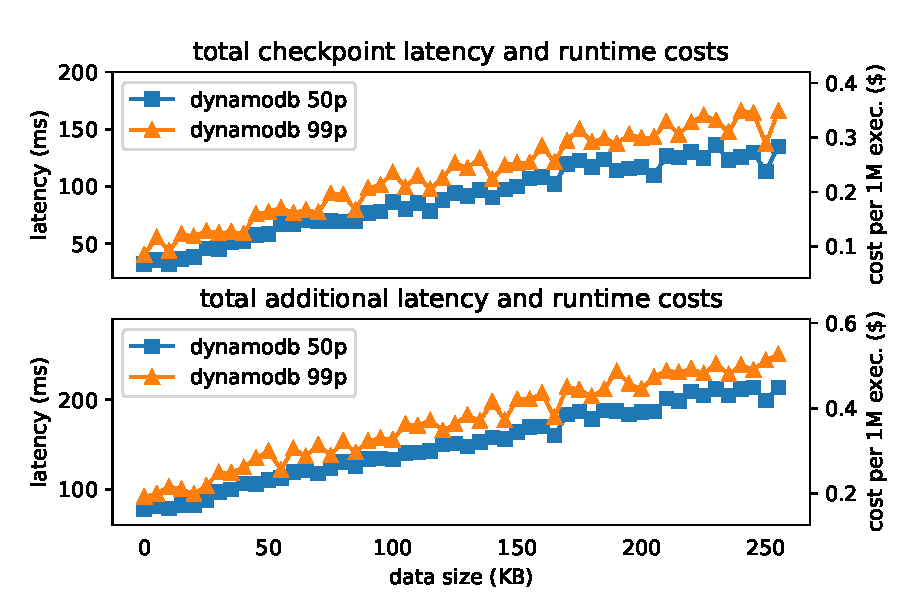
\includegraphics[width=\columnwidth]{figures/TotalAdditionalLatency.pdf}
    % 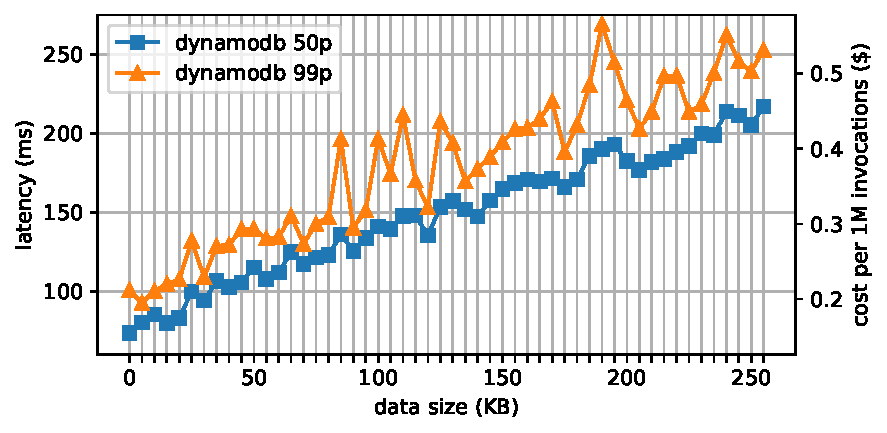
\includegraphics[width=\columnwidth]{figures/TotalAdditionalLatencyNCosts.pdf}
    \caption{Total latency for a transition}
    % \caption{Total latency for a single state transition. We use a
    % chain of two functions (\texttt{F->G}) that simply return their input.
    % \texttt{data size} is the output data size of \texttt{F}, which in turn is
    % the amount of data \texttt{F} writes to checkpoint and the input data size
    % of \texttt{G}.}
    \label{fig:totallatency}
\end{figure}

\begin{figure}[t!]
    \centering
    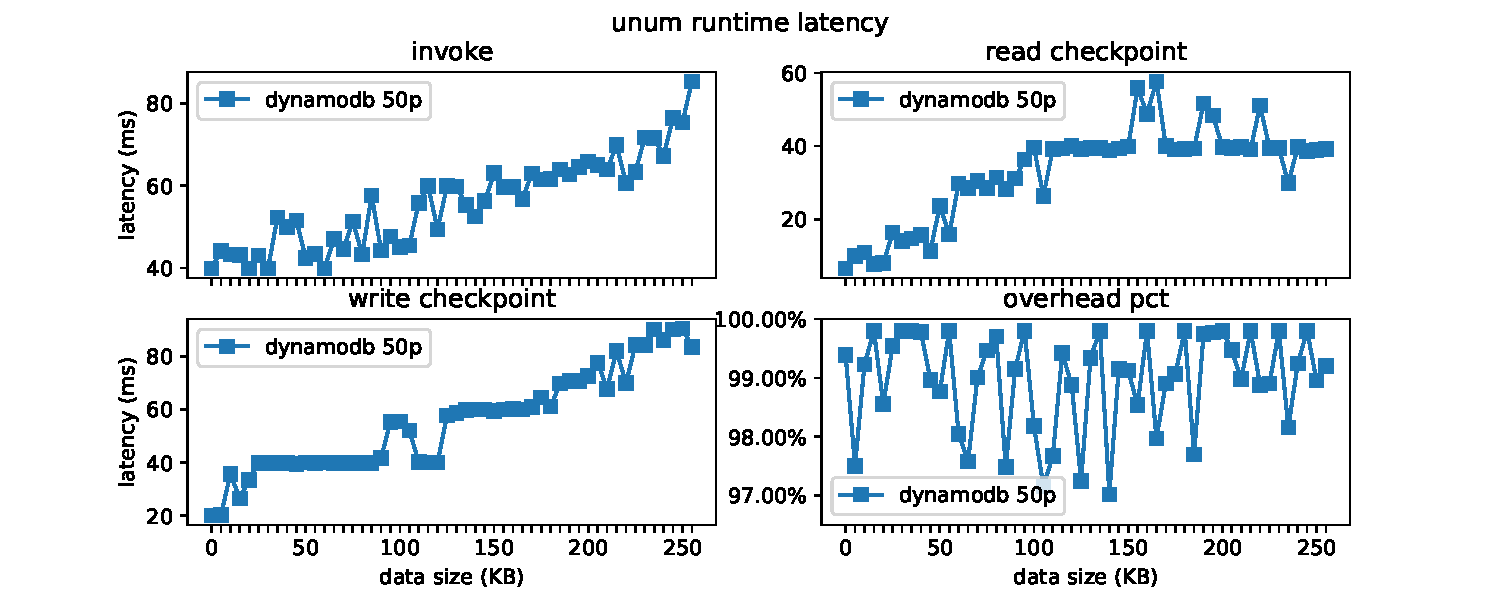
\includegraphics[width=\columnwidth]{figures/OpLatency.pdf}
    \caption{Latency of the Lambda \texttt{invoke} API for triggering a single
    function, the DynamoDB \texttt{GetItem} API for reading a checkpoint and
    the DynamoDB \texttt{PutItem} API for writing a checkpoint}
    \label{fig:oplatency}
\end{figure}

\begin{figure}[t!]
    \centering
    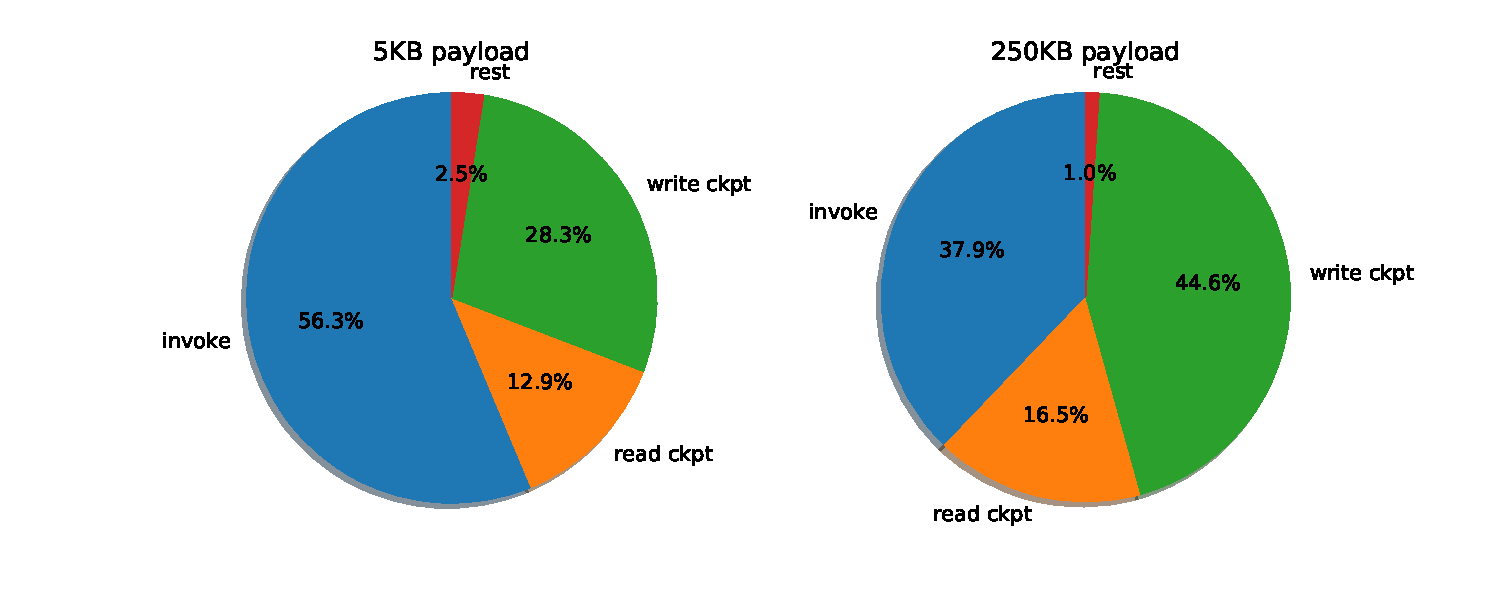
\includegraphics[width=\columnwidth]{figures/OpLatency-pct.pdf}
    \caption{Latency breakdown of the \name{} runtime. The majority of the
    latency comes from API calls to underlying services: the Lambda
    \texttt{invoke}, data store read and write.}
    \label{fig:oplatency-pct}
\end{figure}


% \paragraph{How much additional latency does unum incur? How much does that
% translate to costs?}

\subsubsection{Single transition performance}

A fundamental operation of any serverless workflow system is the transition
between a function's completion and the next function's start. The latency
of transitions bounds the end-to-end performance of workflows. In \name{},
this transition involves (1). writing a checkpoint, (2). invoking the
continuation, and (3). reading a checkpoint. That is two storage accesses and
at least one Lambda \texttt{invoke} call.

Therefore, we start our evaluation by measuring the latency of a single
transition and further breaking it down into the latencies of the Lambda
\texttt{invoke} and data store read and write API calls.

The microbenchmark we use is a chain of two functions (\texttt{F->G}) that
simply return their input without performing any computations. Invoking the
continuation involves a single call to the Lambda \texttt{invoke} API.

Because the latency of storage accesses and the Lambda \texttt{invoke} APIs
depend on how much data is written to the checkpoint and then sent to the next
function as the invocation payload, we measure across data sizes ranging
between 0-255KB in 5KB increments\footnote{Lambda limits payload size to 256KB
for async invocations.}.

As a baseline, we also measure the same latency of a state transition in Step
Functions. However, Step Functions does not generate fine-grained enough logs
for us to measure the exact apple-to-apple comparison. The results we show
measure between a \texttt{LambdaFunctionSucceeded} event and the next
\texttt{LambdaFunctionStarted} event. This is likely an underestimate because
it may not include the latency of persisting function outputs. In fact, based
on end-to-end performance of chaining (Figure~\ref{fig:chainmicrolatency}), it
is almost certain that we are not measuring all of the latency in a state
transition.

Figure~\ref{fig:totallatency} shows the total latency of a transition. \name{}
incurs 73-217ms of latency, depending on the data size. A likely underestimate
of Step Functions latency notwithstanding, \name{} is 1.09-3.54x slower than
Step Functions on a single transition.

Figure~\ref{fig:oplatency} shows the latency of the Lambda \texttt{invoke}
API, the DynamoDB \texttt{GetItem} call to read a checkpoint and the DynamoDB
\texttt{PutItem} call to write a checkpoint. Overall, all three operations
slows down as data size increases.

Figure~\ref{fig:oplatency-pct} shows the latency breakdown for 0KB data size
and 255KB data size. Over 97.5\% of the latency comes from APIs call to Lambda
and data stores. \name{} runtime code only incurs less than 2.5\% of the total
overhead. This means the bulk of \name{}'s performance will automatically
improve with the underlying platform (e.g., a faster Lambda or data store)
without any modification to \name{} itself.

\begin{figure}[t!]
    \centering
    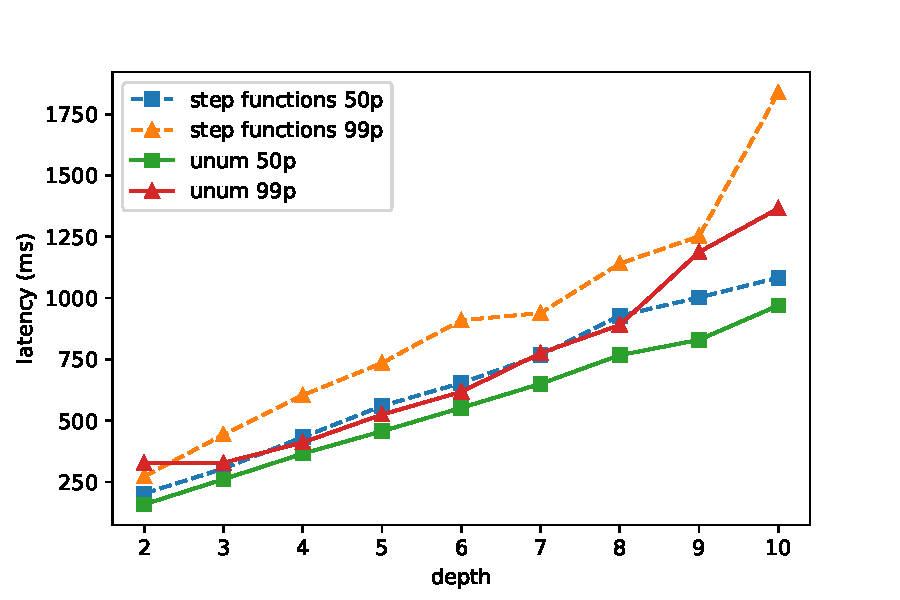
\includegraphics[width=\columnwidth]{figures/ChainMicroLatency.pdf}
    \caption{End-to-end latency of chaining N functions. Lower is
    better. Each function simply returns the input data without performing any
    computation. Results in the figure are for 1KB of input data.}
    \label{fig:chainmicrolatency}
\end{figure}

\begin{figure}[t!]
    \centering
    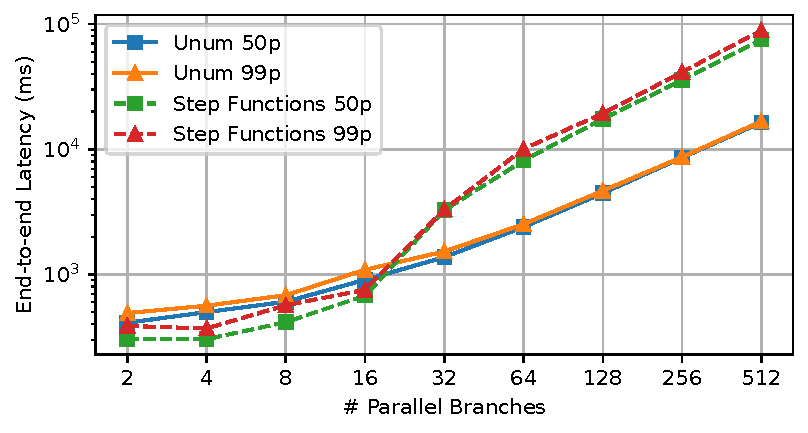
\includegraphics[width=\columnwidth]{figures/MapMicroLatency.pdf}
    \caption{End-to-end latency (logscale) of parallel fan-out and fan-in}
    \label{fig:mapmicrolatency}
\end{figure}

\subsubsection{Chaining performance}

In this section, we discuss how \name{} performs on a basic orchestration
pattern: chaining. Similarly, we use a function that simply returns its input
without any computations in this microbenchmark to minimize the runtime of
user code so that the end-to-end latency maximally reflects the performance of
the workflow system. The workflow consists of a sequential chain of the
function. We experiment with chains of varying length between 2 and 10.

Figure~\ref{fig:chainmicrolatency} shows the end-to-end latency of Step
Functions and \name{} with DynamoDB for input data size of 1KB. We also run
the same microbenchmark with 5KB and 50KB input size and the results are
similar. Overall, \name{} is around 11-28\% faster in chaining than Step
Functions.

\subsubsection{Fan-out and fan-in performance}

Next, we evaluate another critical orchestration primitive: fan-out and
fan-in. Quickly creating parallel instances is an important operation for
serverless because many applications migrate to serverless for its faster
scalability.

Step Functions has two state types, \texttt{Map} and \texttt{Parallel}, for creating
parallel branches. \name{} supports both. This microbenchmark uses the
\texttt{Map} state because it allows easy control on the number of parallel
branches.

Similarly, we use a function that simply returns its input without any
computations in this microbenchmark to minimize the runtime of user code so
that the end-to-end latency maximally reflects the performance of the workflow
system.

Figure~\ref{fig:mapmicrolatency} shows the end-to-end latency (logscale) of
fan-out and fan-in at varying levels of parallelism. At lower level of
parallelism (2-16 parallel branches), \name{} is around 100-200ms slower than
Step Functions. \name{} starts to outperform Step Functions at even moderate parallelism level of 32
parallel branches (2.37x) and up to 4.58x at 512 parallel branches.

As we do not have direct access to Step Functions's backend, it is difficult to
understand why Step Functions's performance becomes worse at higher parallelism. One
possible cause of higher latency is throttlng of concurrent branch creations.
Step Functions documentation states that it might pause creating branches when the
fan-out size exceeds 40~\cite{aws-step-functions-map-state}.

Our result is not arguing that orchestrator-based workflow systems
fundamentally scales worse than \name{}. Although Step Functions does not
elaborate on the reason for throttling, there is little reason to believe that
the maximum allowable concurrency must be capped around 40 for parallel
workloads.

However, this result does demonstrate an important downside of relying on
supplemental services to support serverless workflows. Any services added must
also perform well compared with the highly scalable FaaS engine, otherwise
application developers have to work with the restrictions that the services
impose. \name{} avoids the difficulty of building and maintaining hosted
orchestrators and directly leverages the scalability of Lambda to achieve
better parallel performance.

\subsubsection{Cost comparison}

\begin{figure}[t!]
    \centering
    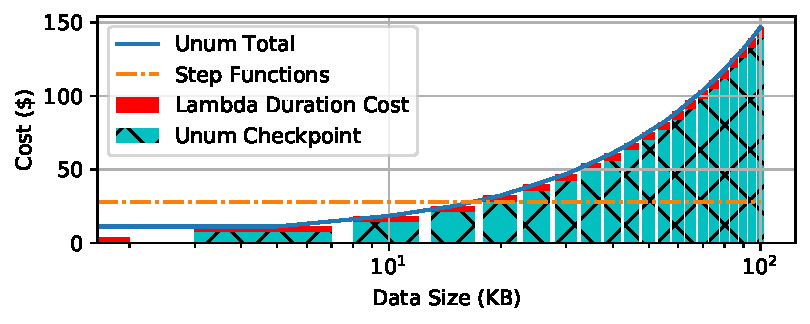
\includegraphics[width=\columnwidth]{figures/TotalCost.pdf}
    \caption{Total costs comparison of 1 million state transitions between
    Step Functions and \name{}. Computation assumes Lambda size of 3GB.}
    \label{fig:total-costs-single}
\end{figure}

\begin{figure}[t!]
    \centering
    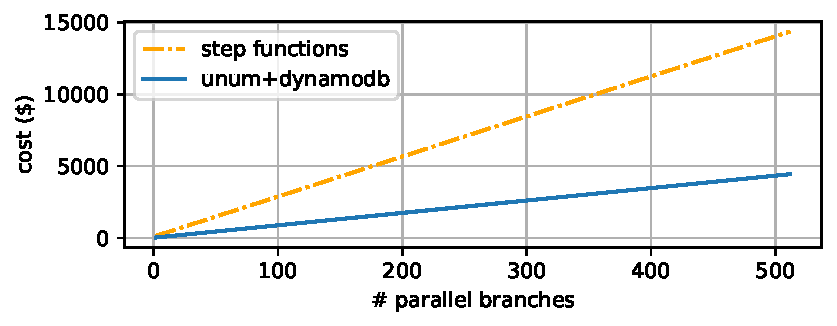
\includegraphics[width=\columnwidth]{figures/TotalMapCost.pdf}
    \caption{Total costs comparison of fan-out and fan-in between Step
    Functions and \name{}. Computation assumes Lambda size of 3GB and 1KB data
    size for function outputs and checkpoints.}
    \label{fig:total-costs-map}
\end{figure}



In this section, we break down the cost of running workflows with \name{} and
compare with that of Step Functions. We discuss the costs for a single transition,
chaining and fan-out.

Costs numbers are calculated based on AWS pricing for \texttt{us-west-1}
region. We do not "measure" the cost of running workflows because AWS does not
provide real-time billing data. We scale costs numbers by 1 million to ease
reading.

Step Functions charges based on the number of state
transitions~\cite{aws-step-functions-pricing}. Each state transition is charged
a fixed rate of \$27.9 $ \times 10^{-6}$.

There are two parts to \name{}'s costs: (1). additional Lambda duration
billing for running the \name{} runtime, and (2). data store reads and writes.

We do not count the storage costs in the intermediary data store because after
a workflow execution, checkpoints can be immediately deleted or moved to
cheaper storage by the user.

Figure~\ref{fig:total-costs-single} shows the total cost of transitions for
function data size varying between 0-255KB. The computation assumes Lambda
memory size of 3GB. We can see that the additional Lambda duration costs from
running \name{} runtime is a small fraction when compared with the costs of
DynamoDB writes. In fact, even at 255KB, the additional Lambda
duration costs is only abour \$10. If using the smallest 128MB lambdas, the
costs diminishes to merely \$0.46.

DynamoDB writes dominates the costs in \name{} because the on-demand mode
charges only not on the number of writes but also on the amount of data
written. For 1KB of data, DynamoDB charges $1.3942 \times 10^{-6}$ for a write
and $0.279 \times 10^{-6}$ for a read. Because checkpoint reads do not return
any data when there are no faults, the cost of checkpoint reads does not
increase with the data size and stays merely \$0.279 for the computation in
Figure~\ref{fig:total-costs-single}.

Even though the simulation in Figure~\ref{fig:total-costs-single} shows the
costs of \name{} outpacing that of Step Functions at larger data sizes, our
macrobenchmark results demonstrate that functions in real-world serverless
workflows do not output large amount of data. In fact, workflows tend to use
their own storage and manage application data manually. Checkpoints in the
\name{} intermediary data store are normally under 1KB.

Figure~\ref{fig:total-costs-map} shows the total costs of fan-out and fan-in
when function checkpoints are under 1KB. In addition to the costs discussed
for a single transition, the entry function performing the fan-out incurs
higher Lambda duration costs for invoking each fan-out function. The fan-in
function at the end also causes extra costs because it reads the checkpoints
of all fan-out branches. However, the total costs of this microbenchmark is
more than 3.2x lower with \name{} than Step Functions.

% \begin{itemize}

%     \item S3 charges \$5.5 per 1M PUT requests (for checkpoint write) and \$0.44
%     per 1M GET requests (for checkpoint read).

%     \item DynamoDB on-demand capcity mode charges reads and writes based on
%     the data size. 1M requests for writing 1KB data costs \$1.3942 and 1M
%     requests for reading 1KB data costs \$0.279. Note that in the case of
%     DynamoDB, if no faults happen during execution, the checkpoint read will
%     return "item not found", which costs the same as returning 1KB of data.

%     \item For 1M state transitions, \name{}'s costs for S3:

%     \[  r(d)\times0.05 + 5.94 \]

%     and for DynamoDB:

%     \[  r(d)\times0.05 + d\times1.3942 +0.279\],

%     where $r$ is the total additional runtime of \name{}, $d$ is the data
%     size.

% \end{itemize}




\subsection{Macrobenchmarks}

% \begin{table}[]
% \begin{tabular}{llllll}
% \hline
%                      &                        & \multicolumn{2}{l}{\textbf{unum}}                                                                                                   & \multicolumn{2}{l}{\textbf{Step Functions}}                                                                     \\
% \textbf{Application} & Pattern                & \textit{e2e latency} & \textit{cost (per 1M exec.)}                                                                                 & \textit{e2e latency} & \textit{cost (per 1M exec.)}                                                             \\ \hline
% IoT Pipeline         & chain                  & 120.9ms              & $0.2*2+(73+28)*$0.0021+2*\$1.3942                                                                            & 226.52               & $0.2*2+ 4*$27.9                                                                          \\
% Text Processing      & fan-out, fan-in        & 562.69ms             & $0.2*6+ (105+149+70+68+144+100)*$0.0021 + 6*$1.3942+2*2*$0.279                                               & 552.46ms             & $0.2*5+7*$27.9                                                                           \\
% Wordcount            & chain, fan-out, fan-in & 410s                 & $0.2*(1+262+1+250+1) + (277+6264*262 + 348 + 667*250 +68)*$0.0021 +(1+262+1+250+1)*$1.3942 + 262*2*$0.279+ 250*2* $0.279    & 898s                 & $0.2*(1+262+1+250+1) + (5913*262 + 154 + 633*250 +5)*$0.0021 +(1+262+1+1+250+1+1)*\$27.9 \\
% ExCamera             & chain, fan-out, fold   & 84s                  & $0.2*(1+16+15+15+14) + (6500+1500+350+4500+5000)*$0.0021+ (1+16+15+15+14)*$1.3942 + 15*2*$0.279+14*2*\$0.279 & 98s                  & $0.2*(16+16+1+16+15)+(6300+1400+2+5500+5300)*$0.0021+(1+16+16+1+1+16+1+1)*\$27.9      \\ \hline
% \end{tabular}
% \end{table}

\begin{table*}[t]
\centering
\begin{tabular}{ll|cc|cc}
\hline
                     &                        & \multicolumn{2}{c}{\textbf{\name{}}}            & \multicolumn{2}{c}{\textbf{Step Functions}}       \\
\textbf{Application} & \textbf{Pattern}       & \textit{e2e latency} & \textit{cost (per 1 mil. exec.)}   & \textit{e2e latency} & \textit{cost (per 1 mil. exec.)}            \\ \hline
IoT Pipeline         & chain                  & 120.9ms              & \$3.4005      & 226.52       & \$111.6    \\
Text Processing      & fan-out, fan-in        & 562.69ms             & \$12.0168      & 552.46ms             & \$196.3                                                                           \\
Wordcount            & chain, fan-out, fan-in & 410s                 & \$4904.79   & 898s                 & \$18113 \\
ExCamera             & chain, fan-out, fold   & 84s                  & \$150.91 & 98s                  & \$1530      \\ \hline
\end{tabular}
\caption{Latency and costs comparison between \name{} and Step Functions for the macrobenchmark applications}
\label{table:macro}
\end{table*}

We further evaluate \name{}'s performance, costs and expressiveness with 4
real-world applications. 

\paragraph{IoT Pipeline} Adapted from a humidity control application in the
AWS serverless repository~\cite{iot-pipeline}. The workflow consists of a
chain of two functions that processes climate control data and change the HVAC
setting.

\paragraph{Text Processing} Adapted from the social network application in
DeathStarBench~\cite{deathstar}. The workflow consists of 5 functions that
create a social network post by processing user mentions, shortening URLs and
eventually saving the post in a DynamoDB table.

\paragraph{Wordcount} MapReduce word count~\cite{mapreduce} ran with 250
parallel mappers and reducers.

\paragraph{ExCamera} The ExCamera video encoder~\cite{excamera, gg-atc}. We
use the same workload and setup as the experiment in gg~\cite{gg-atc}: the same
input video of the first 888 chunks of sintel 4K, 3GB lambdas and 16 chunks
per batch.

Table~\ref{table:macro} lists the median end-to-end latency and computed costs
per 1 million executions. Both latency and costs numbers are based on DynamoDB
as the intermediary data store. \name{} is slower than Step Functions for Text
Processing where the workflow fans out to 2 parallel branches. However,
\name{} is faster in the other applications that consists of chaining and
fan-outs at much higher level of parallelism.

Furthermore, \name{} is consistently cheaper than Step Functions for all
workloads with 3.7x to 32.8x costs savings. Most applications manually manage
application data with their own storage and function checkpoints are smaller
than 1KB for all 4 workflows.

\subsubsection{ExCamera}\label{sec:eval-excamera}

\begin{itemize}

    \item \name{} is able to express and execute parallel pipelines while Step
    Functions has to serialize the decode and re-encode stages.

    \item Step Functions does not have a way to express fold, so the last
    rebase stage has to be written as a single recursive function. \name{}
    supports fold. The recursion logic is lifted to the \name{} IR and the
    rebase function is written similarly to ExCamera.

    \item \name{} is 7.1\% faster than gg's implementation of ExCamera and
    \%10.5 slower than the original ExCamera. Similar to gg, \name{} also do
    not pre-load the input data from S3. Different from gg, \name{} does not
    use a long-running coordinator on EC2 to manage communications and
    invocations.

\end{itemize}

\subsubsection{Questions}

\begin{enumerate}

    \item How do we evaluate and present execution guarantee? Anything to show
     to convince our reader that it's correct?

    \item How do we evaluate other benefits that stem from a simpler design
     (the fact that unum gets rid of the needs for a separate orchestrator
     service), such as resource management, required staffing and other
     hosting costs? Further on the resource utilization point, do we want to
     say that dollar costs of running applications is a reasonable enough
     proxy to resource consumption and therefore lower price = less resource
     consumption = better resource utilization?

    \item Should we run experiments with S3 and present those numbers?

    \item How to discuss the expressiveness advantage? Specifically,

        Step Functions has no way to express a for loop or fold.

        Step Functions has no way to express pipeline parallelism.

        Step Functions fan-in needs to make sure the aggregate data doesn't exceed a
        limit, unum automatically passes data in using pointers to the intermediary
        data store.

\end{enumerate}


\section{Related Work}\label{sec:related}

Overall characteristics of orchestrator based engines: The orchestrator
performs function invocations; functions send results back to correct the
orchestrator instance.

Why does this characterstics matter?

Questions:

\begin{itemize}
	\item Is it pure serverless? What does pure serverless mean?
	\item Any performance comparisons necessary?
\end{itemize}

\paragraph{gg}~\cite{gg-atc}

\begin{itemize}
	\item Target applications are what they call "everyday tasks", including code compilation, unit testing, video encoding and object recognition
	\item A thunk = a x86-64 executable and its input data

	A thunk is deterministic. Forcing a thunk multiple times will generate the same object.

	Data objects are named (naming scheme 3.1.1). Reading an object might involve forcing a thunk to generate the object. A thunk's input can be references to other thunk's outputs. gg uses this mechanism to express computation graphs.

	Forcing a thunk multiple time will always produce the same object with the same name. To run the same function with different input needs to define a different thunk (presumably a gg compiler can help simplify the step of defining thunks that have the same executable and different input. But the paper wasn't entirely clear on this and the source code shows application-specific compilation with limited programmability.).


	duplicate functionalities that Lambda already provides: job scheduling, retry, timeouts.



\end{itemize}


\paragraph{Triggerflow}~\cite{triggerflow}
See Section 4. implementation. Each workflow has its own workflow worker which is really a kubernetes pod. The workflow works process events and trigger actual FaaS functions.


\paragraph{Kappa}~\cite{kappa}
Tasks communicate with the coordinator through
the remote procedure calls (RPCs) summarized in Table 2


\paragraph{Cloudburst}~\cite{cloudburst}
1. Orthogonal: They focus on building a data store with specialized APIs and consistency models for faas workflow
2. Differennt programming interface (TODO: more details)
3. Not built on real faas platform; can't run on aws, azure or google cloud


\paragraph{mu and Excamera}~\cite{excamera}

\paragraph{Boki}


\paragraph{PyWren}~\cite{pywren}



% Google Cloud Composer uses Airflow.
% https://github.com/apache/airflow/tree/main/airflow/example_dags
% https://cloud.google.com/composer/docs/samples

% Azure Durable Functions. https://docs.microsoft.com/en-us/learn/modules/create-long-running-serverless-workflow-with-durable-functions/

% Google Cloud Workflows.
% Example: https://codelabs.developers.google.com/codelabs/cloud-workflows-intro
% https://cloud.google.com/workflows
% Repository: https://cloud.google.com/workflows/docs/samples

 
% https://github.com/serverlessworkflow/specification/tree/main/examples



% https://github.com/kalevalp/hello-retail-baseline
\section{Limitations \& Future Work}\label{sec:limitations}

\paragraph{Unsupported applications.} \name{} supports a superset of
applications that can be expressed using Step Functions, but there are
applications that do not fit \name{}'s constraints. In particular, \name{} only
supports statically defined control structures. For example, Durable Functions
expresses workflows dynamically as code and allows the developer to use
arbitrary logic to determine what the next workflow step should be at runtime.
This is not currently possible with \name{}.

\paragraph{Measurement error.} Due to the opaque design, implementation and
pricing of production workflow systems, such as Step Functions, comparisons in
our evaluations are limited in their explanatory power. In particular, we use
the current \emph{price} of Lambda, DynamoDB, and Step Functions as a proxy for
the \emph{cost} of providing these services. Of course, different platform
providers may choose different pricing schemes and prices may be either lower or
higher for a particular service than the underlying cost.

Similarly, performance measurements of Step Functions is done as a black box and
thus cannot determine which components of performance are due to design choices
(such as requiring additional network communication) and which are due to
deployment variables (queue depth, provisioned resources, etc).

\paragraph{Support for more languages and platforms.} While \name{} is designed
to run on any serverless platform that meets our minimal criteria, our current
implementation is only complete for AWS Lambda using DynamoDB or S3 for storage.
We are working on other backends, including for Azure Functions and Google
Functions, allowing the same applications to run on multiple platforms.

Moreover, we only described a front-end compiler that targets the Step Functions
description language. We intend to implement compilers for other workflow
description languages as well.

\section{Conclusion}\label{sec:conclusion}

Serverless platforms allow developers to construct applications from modular
programming units that can scale quickly and independently, promising
burst-scalability and fine-grained billing. Workflow orchestrators make building
complex applications out of these event-driven, asynchronous functions
reasonable, but may introduce performance, cost, scalability, and deployment
overhead to developers and platform providers. We designed and implemented
\name{}, a \emph{decentralized} workflow orchestrator that requires no
additional infrastructure to deploy, imposes no additional limits on
scalability, and performs as well as or better than centralized solutions while
providing similar expressiveness and execution guarantees.

\setlength{\parindent}{0pt}
% The value of \verb|\parskip| is \texttt{\the\parskip}
\setlength{\parskip}{1pt plus2pt}
% The value of \verb|\parskip| is \texttt{\the\parskip}
\par
\textbf{Acknowledgments} We thank the anonymous reviewers and our shepherd,
Douglas Terry, for their insightful comments. We thank Landon Cox for his
support and feedback during the early stage of this project. This work was
funded in part by NSF Grant 2028869.
%-------------------------------------------------------------------
% \vspace{5in} % TODO remove this later, just for dodging strange latex error messages caused by bugs in page breaking bibliography
\setlength{\parindent}{10pt}
\setlength{\parskip}{0pt plus1pt}
\bibliographystyle{plain}
\bibliography{references}

%%%%%%%%%%%%%%%%%%%%%%%%%%%%%%%%%%%%%%%%%%%%%%%%%%%%%%%%%%%%%%%%%%%%%%%%%%%%%%%%
\end{document}
%%%%%%%%%%%%%%%%%%%%%%%%%%%%%%%%%%%%%%%%%%%%%%%%%%%%%%%%%%%%%%%%%%%%%%%%%%%%%%%%

%%  LocalWords:  endnotes includegraphics fread ptr nobj noindent
%%  LocalWords:  pdflatex acks
